%----------------------------------------------------------------------------------------
%	CHAPTER 3
%----------------------------------------------------------------------------------------
\chapterimage{chapter_head_2.pdf} % Chapter heading image

\chapter{Sistemas de Equações Lineares}
\section{Sistemas de Equações Lineares}\index{Sistemas de Equações Lineares}

\subsection{Equações Lineares}

Para iniciar o capítulo é importante definir alguns pontos. O leitor nesse momento pode lembrar, da disciplina Matemática, que \textit{funções lineares} são aquelas que resultam em um gráfico no formato de reta, costumeiramente chamadas de \textit{linha}. Vendo o exemplo abaixo é possível retomar, rapidamente, o gráfico de uma função linear.
\begin{example}
	\video \, Construa o gráfico da função $f(x)=2x +1$.


	Analisando a função dada, é possível definir algumas coisas através da comparação com a definição geral de funções lineares:
	
	\begin{align*}
		f(x) & =  a\cdot x+b\quad\mathrm{Defini\text{\c{c}}\tilde{a}o\,\,geral}\\
		f(x) & =  2\cdot x+1\quad\mathrm{Fun\text{\c{c}}\tilde{a}o\,\,do\,\,enunciado}
	\end{align*}
	
	- $x$: variável independente;
	
	- $f(x)$ ou $y$: variável dependente;
	
	- $f$: nome da função;
	
	- $a$: coeficiente angular. Define o ângulo entre a reta (função) e o \textit{eixo das abscissas}, também chamado de \textit{eixo horizontal} ou, ``popularmente'', \textit{eixo x} \footnote{Existem alguns pontos a serem considerados aqui: 1) quando é falado \textit{eixo horizontal} podem haver interpretações erradas pois é uma questão de referência, ou seja, se o leitor girar o papel em
		90\textdegree , o eixo se tornará vertical! Chamar de \textit{eixo x} também podem haver interpretações diferenciadas, pois se o problema trata de uma situação onde envolva o cálculo do espaço de um móvel ($S$) em função do tempo ($t$), essa nomenclatura não fará sentido algum. O modo correto de interpretar e nomear o eixo é utilizar \textit{eixo das abscissas} ou, se o leitor preferir, pode utilizar o nome da variável independente para o nome do eixo, ou seja, no mesmo exemplo anterior, cálculo do espaço em função do tempo, pode ser utilizado para o \textit{eixo das abscissas} simplesmente \textit{eixo de t} ou \textit{eixo do tempo}.}. Se $a > 0$ a função é crescente; se $a<0$ a função é decrescente; se $a=0$ a função é constante;
	
	- $b$: coeficiente linear. É o valor que \text{intercepta}, ou\textit{"corta"} o \textit{eixo das ordenadas}, conhecido também como \textit{eixo vertical}, ou ainda como \textit{eixo y} \footnote{Mesma consideração da nota anterior.}.
	
	Desse modo para fazer o gráfico é necessário apenas dois pontos, ou seja, dois \textit{pares ordenados }$(x,f(x))$. Um desses pares pode
	ser obtido através do coeficiente linear, ou seja, se a função intercepta o eixo das ordenadas no valor 1 ($b=1$), necessariamente, $x=0$,
	assim $(0,1)$ é um ponto (ponto vermelho). A determinação de outro ponto pode ser atribuindo um valor, diferente de zero, para a variável
	independente e calcular seu correspondente. Atribuindo $x=1$ tem-se $f(1)=2\cdot 1 + 1 \Rightarrow f(1)=3$ logo, o segundo ponto (ponto
	preto) será $(1,3)$. Unindo esses dois pontos e traçando uma reta é possível obter o gráfico abaixo:

\begin{figure}[H]
	\caption{Gráfico de uma função linear}
	\begin{center}
		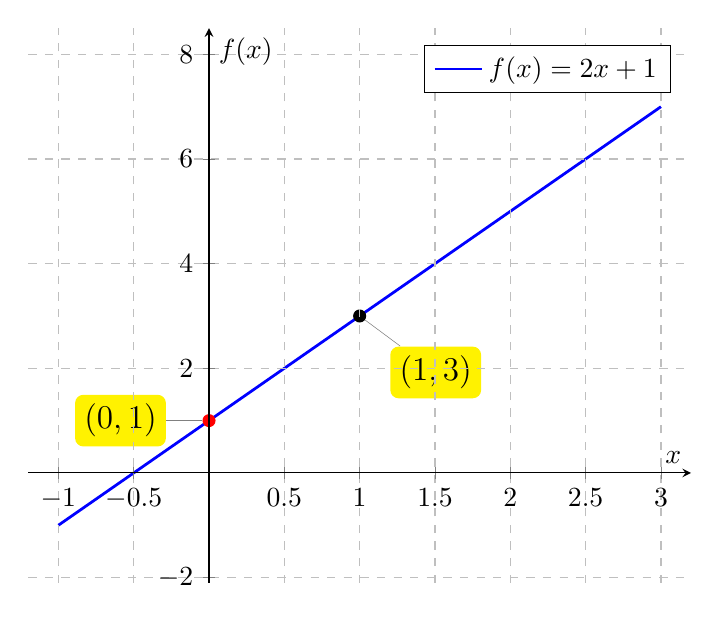
\begin{tikzpicture}[scale=1.0]
		% Estilos
		\tikzstyle {every pin} = [ fill=yellow!100!white, rectangle, rounded corners=3pt, font=\large ]
		\begin{axis}
			[
				grid, grid style=dashed,
				grid = both,
				ymin=-2.1,ymax=8.5,
				xmin=-1.2,xmax=3.2,
				xlabel=$x$,
				ylabel=$f(x)$,
				width=10cm,
				axis on top=true,
				axis x line=middle,
				axis y line=middle,
				%transpose legend,
				%legend columns = 1,
				%legend style = {at={0.5,-.1},anchor=north}
				legend pos= north east, %outer
			]
		% Desenha a função
			\addplot [blue,line width = 1, smooth, domain=-1:3] {2*x +1}; \addlegendentry{x}
		
		% Pontos de interesse
			\node [fill=black, circle, scale=0.5, pin=-45:{$(1,3)$}] at (axis cs: 1,3) {};
			\node [fill=red, circle, scale=0.5, pin=180:{$(0,1)$}] at (axis cs: 0,1) {};
			%\node [fill=blue, circle, scale=0.1, pin=135:{$f(x)=2x+1$}] at (axis cs: 2.75,6.5) {};
			\legend {$f(x)=2x+1$}
		\end{axis}
		\end{tikzpicture}
	\end{center}
	\label{fig:funcao_linear}
	%\vspace{-1cm}
	%\begin{center}
	%\makebox[\width]{Legenda}
	%\end{center}
	\hspace{1.5cm}\makebox[\width]{Fonte: Próprio autor.}
\end{figure}

\doutor \url{https://www.youtube.com/watch?v=KreVo3UpTzM}
\end{example}


Como pode ser visto na Figura \ref{fig:funcao_linear}, o gráfico da função do exemplo anterior é uma reta pois os expoentes das variáveis,
independente e dependente são iguais a 1. A função do exemplo anterior pode ser reescrita para a forma:

$$
y-2x=1
$$

A forma como a função foi reescrita pode ser entendida como uma \textit{equação linear}. De modo geral sobre \textit{Equações Lineares} são equações do tipo:

$$
a_{1}x_{1}+a_{2}x_{2}+a_{3}x_{3}+\cdots+a_{n}x_{n}=b
$$

onde $a_1, a_2, a_3, \ldots, a_n$ são os coeficientes, $x_1, x_2, x_3, \ldots, x_n$ são as variáveis e $b$ é o termo independente.
\begin{example}
	A equação $2x + 3y -4z = 2$ é uma equação linear. Seus coeficientes são $2,3\, \mathrm{e}\,-4$. Já as variáveis são $x,y\, \mathrm{e}\, z$
	e 2 é o termo independente. A solução para esta equação ocorre quando $x=3, y=0\, \mathrm{e}\,z=1$ pois $2\cdot 3+3\cdot 0 -4 \cdot 1 = 2$.
\end{example}
%
\begin{example}
	Verifique se $(1,2,0)$ e $(1,0,0)$ satisfazem a equação linear $2x+3y-4z=2$.

	Para verificar se as triplas\footnote{Um nome mais apropriado para chamar um conjunto de valores, ordenados, é utilizando a quantidade de elementos dessa organização, ou seja: 2 valores implicam numa dupla ou par ordenado; 3 valores, tripla ordenada; 4 valores, quadrupla ordenada; 5 valores, quíntupla ordenada; ``n'' valores n-upla (ênupla).} ordenadas satisfazem a equação linear basta substituir os valores
	dados em suas respectivas variáveis, assim:

\begin{itemize}
	\item $(1,2,0)\Rightarrow 2\cdot 1 +3 \cdot 2 -4 \cdot 0 = 2 \Rightarrow 2+6-0=2 \Rightarrow 8=2\,\,\,\mathrm{FALSO}$.
	Logo, a $(1,2,0)$ não satisfaz a equação linear do enunciado.
	\item $(1,0,0)\Rightarrow 2\cdot 1 +3 \cdot 0 -4 \cdot 0 = 2 \Rightarrow 2+0-0=2 \Rightarrow 2=2\,\,\,\mathrm{VERDADEIRO}$.
	Logo, a $(1,0,0)$ satisfaz a equação linear do enunciado.
\end{itemize}
\end{example}
%
O leitor pode imaginar que as equações lineares acima existam infinitas combinações entre valores numéricos que satisfaçam a relação. Isso
acontece porque o \textit{número de variáveis} é MAIOR que o \textit{número de equações}. No entanto, existem situações em que o número de equações lineares é igual ao número de variáveis.
\begin{example}
	\video \, Dado as funções Receita ($R(x)=30x$) e Custo ($C(x)=20x+1000$),
	determine o ponto de equilíbrio\footnote{O ponto de equilíbrio acontece quando a Receita é igual ao Custo,
		ou seja, $R(x)=C(x)$}.

	Para determinar o ponto de equilíbrio basta fazer $y=R(x)=C(x)$ e substituir nas equações do enunciado, assim:
\begin{itemize}
	\item Função Receita: $y=30x$;
	\item Função Custo: $y=20x+1000$.
\end{itemize}
Fica claro a existência de duas equações (Receita e Custo) e duas variáveis ($x\,\mathrm{e}\,y$). A solução dessas equações lineares devem satisfazer as duas funções simultaneamente, desse modo, é possível escrever um \textit{sistema de equações lineares}, como segue:

\begin{ceqn}
	\begin{align*}
	\left\{ \begin{alignedat}{1}\begin{array}{ccc}
	y & = & 30x\\
	y & = & 20x+1000
	\end{array}\end{alignedat}
	\right. & \Leftrightarrow\\
	\left\{ \begin{alignedat}{1}\begin{array}{ccc}
	y-30x & = & 0\\
	y-20x & = & 1000
	\end{array}\end{alignedat}
	\right. & \Leftrightarrow\\
	\left\{ \begin{alignedat}{1}\begin{array}{ccc}
	y-30x & = & 0\\
	-10x & = & -1000
	\end{array}\end{alignedat}
	\right. & \Rightarrow  x=100\\
	y-30\cdot100=0 & \Rightarrow\\
	y-3000=0 & \Rightarrow  y=3000
	\end{align*}
\end{ceqn}


Assim, o ponto de equilíbrio é $(100,3000)$ e representa a quantidade de produtos que devem ser vendidos ($x=100\,\,\mathrm{unidades}$)
e o valor da Receita e do Custo quando forem vendidos $x=100$ produtos será de R\$3000,00 ($y=3000\Rightarrow R(100)=C(100)=\mathrm{R}\$ \,3000,00$).
A Figura \ref{fig:sistema_linear} mostra o gráfico das funções e o ponto de equilíbrio.

\begin{figure}[H]
	\caption{Gráfico das funções Receita e Custo}
	\center 
	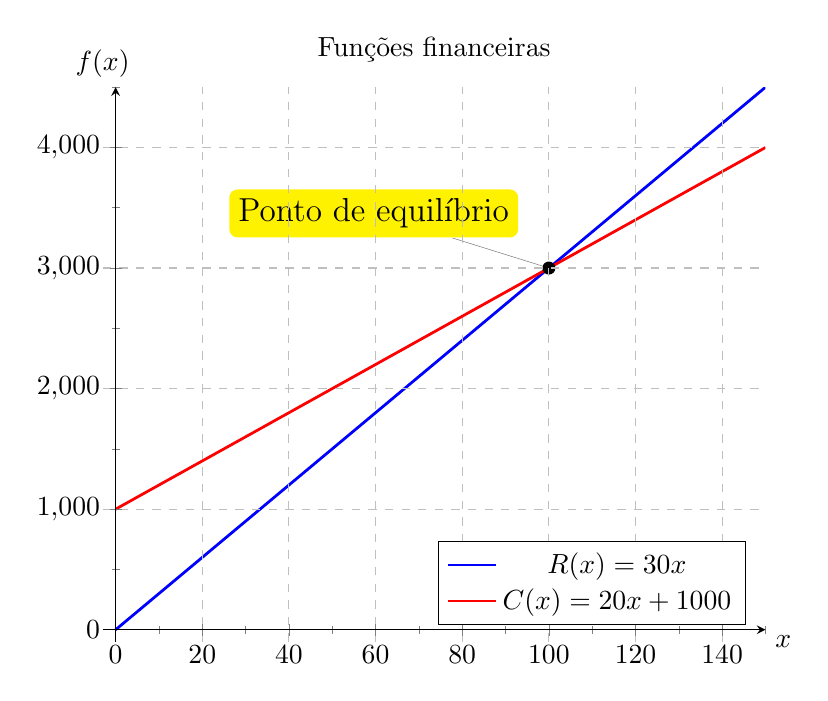
\begin{tikzpicture}[scale=1.0] 	% The Styles 	
	\tikzstyle {every pin} = [ fill=yellow!100!white, rectangle, rounded corners=3pt, font=\large ] 	
	\begin{axis} 		
	[ 		
	title=Funções financeiras,
	grid, grid style=dashed,
	extra y ticks={0},
	extra x ticks={0},
	set layers, 		
	ymin=-100,ymax=4500, 		
	xmin=-3,xmax=150, 			
	width=10cm, 		
	grid=major,		%%both
	minor tick num=1,		
	axis on top,		%%retirado =true 	
	axis lines=middle, 		
	legend pos= south east,
	xlabel=$x$, 		
	ylabel=$f(x)$,
	x label style={at={(1,0)},right},
	y label style={at={(0,1)},above},
	x tick label style={/pgf/number format/.cd, fixed relative, },		
	] 	%Draw the function 	
	\addplot [blue,line width = 1, smooth, domain=0:150] {30*x}; 	
	\addplot [red,line width = 1, smooth, domain=0:150] {20*x+1000}; 	
	% And now the interesting point 	
	\node [fill=black, circle, scale=0.5, pin=135:{Ponto de equilíbrio}] at (axis cs: 100,3000) {};
	\legend {$R(x)=30x$,$C(x)= 20x+1000$} 	
	\end{axis} 
	\end{tikzpicture} 
	\center	
	\label{fig:sistema_linear}
	\hspace{-1cm}\makebox[\width]{Fonte: Próprio autor.}
\end{figure}


\doutor \url{https://www.youtube.com/watch?v=8mZ7W4jwPWY}
\end{example}

Como visto anteriormente, os sistemas de equações lineares podem ser aplicados na área da Administração, Ciências Contábeis e, é claro, na área de exatas!

Desse modo é de fundamental importância saber resolver os sistemas de equações lineares e, para isso, existem alguns métodos. Será visto
aqui o método da resolução usando matrizes, chamada de regra de Cramer e o método da eliminação de Gauss.

Antes de conhecer as técnicas é importante frisar que os sistemas de equações lineares podem ser classificados dependendo do número de soluções que o mesmo apresenta:

\begin{itemize}
	\item \textbf{Sistema Impossível}: Quando o sistema não admite solução;
	\item \textbf{Sistema Possível e Indeterminado}: Quando o sistema admite
	mais de uma solução;
	\item \textbf{Sistema Possível e Determinado}: É o sistema que possui uma
	única solução possível.
\end{itemize}

\subsection{Regra de Cramer}

Considere o sistema abaixo:

$$
\begin{cases}
\begin{array}{ccc}
x+y+z & = & 6\\
x-y+z & = & 2\\
x+y-z & = & 0
\end{array}\end{cases}
$$

É possível escrever a Matriz Principal deste sistema. A Matriz Principal é composta pelos coeficientes de cada variável do sistema, ou seja

$$
\mathbb{{M}}=\begin{bmatrix}1 & 1 & 1\\
1 & -1 & 1\\
1 & 1 & -1
\end{bmatrix}
$$

Ainda é possível definir as matrizes $\mathbb{M}_x,\,\, \mathbb{M}_y,\,\, \mathrm{e}\,\, \mathbb{M}_z$ substituindo os valores da coluna do resultado nas respectivas colunas da matriz principal, assim:

$$
\mathbb{{M}}_{x}=\begin{bmatrix}6 & 1 & 1\\
2 & -1 & 1\\
0 & 1 & -1
\end{bmatrix},\quad\mathbb{{M}}_{y}=\begin{bmatrix}1 & 6 & 1\\
1 & 2 & 1\\
1 & 0 & -1
\end{bmatrix},\quad\mathbb{{M}}_{z}=\begin{bmatrix}1 & 1 & 6\\
1 & -1 & 2\\
1 & 1 & 0
\end{bmatrix}
$$

Então, o valor das variáveis do sistema dado pode ser calculado através de:

$$
x=\frac{{\mathrm{det}(\mathbb{{M}}_{x})}}{\mathrm{det}(\mathbb{M})},\quad y=\frac{\mathrm{det}(\mathbb{M}_{y})}{\mathrm{det}(\mathbb{M})},\quad\mathrm{e\quad z=\frac{\mathrm{det}(\mathbb{M}_{z})}{\mathrm{det}(\mathbb{M})}}
$$

%\subsection{Método da Substituição}

%O método da substituição consiste em realizar processo de isolamento de variável em uma equação do sistema e substituir em outras equações do sistema.

%...continua...

\subsection{Eliminação de Gauss - Método do escalonamento}

Um sistema de equações lineares pode ser escrito da seguinte forma:

$$
\mathbb{A}\cdot\mathbb{X}=\mathbb{B}
$$

Onde a matriz $\mathbb{A}$ é a matriz dos coeficientes, $\mathbb{X}$ é a matriz das variáveis e $\mathbb{B}$ é a matriz dos resultados.

O objetivo da eliminação de Gauss é formar uma matriz triangular superior. 
Em um sistema de equações lineares é possível fazer:
\begin{itemize}
	\item Multiplicar uma linha inteira por um número diferente de zero;
	\item Mudar a posição das linhas e/ou colunas;
	\item Efetuar operações entre as linhas.
\end{itemize}
\begin{example}
	\video \, Resolva o sistema abaixo
	
	$$
	\begin{cases}
	x+y+z & =3\\
	2x+y+2z & =5\\
	x-y+3z & =1
	\end{cases}
	$$


\solucao

	O sistema do enunciado pode ser escrito através da multiplicação abaixo
	
	$$
	\underbrace{\begin{bmatrix}1 & 1 & 1\\
		2 & 1 & 2\\
		1 & -1 & 3
		\end{bmatrix}}_{\mathbb{A}}\cdot\underbrace{\begin{bmatrix}x\\
		y\\
		z
		\end{bmatrix}}_{\mathbb{X}}=\underbrace{\begin{bmatrix}3\\
		5\\
		1
		\end{bmatrix}}_{\mathbb{B}}
	$$
	
	O próximo passo é montar a chamada \textit{Matriz Ampliada} do passo inicial ou passo zero (0).
	
	$$
		\left[ \mathbb{A}|\mathbb{B}\right ]^{(0)}=\left[ \begin{matrix}1&1&1\\2&1&2\\1&-1&3 \end{matrix} \left| \begin{matrix} 3\\5\\1\end{matrix}\right. \right ]
	$$
	
	Após a definição da Matriz Ampliada, o próximo passo é zerar os elementos que estão abaixo da diagonal principal, assim:
	\[
	\begin{aligned}
	L_2^{(1)} &\leftarrow 2\cdot L_1^{(0)}-L_2^{(0)} \\
	L_3^{(1)} &\leftarrow L_1^{(0)}-L_3^{(0)}
	\end{aligned}
	\]
	
	resultando em:
	\[
	\left[ \mathbb{A}|\mathbb{B}\right ]^{(1)}=\left[ \begin{matrix}1&1&1\\0&1&0\\0&2&-3 \end{matrix} \left| \begin{matrix} 3\\1\\2\end{matrix}\right. \right ]
	\]
	
	O próximo passo é usar a linha 2 como referência para zerar os elementos que estão abaixo da diagonal principal. Assim:
	
	\[
	\begin{aligned}
	L_3^{(2)} &\leftarrow 2 \cdot L_2^{(1)}-L_3^{(1)}
	\end{aligned}
	\]
	
	obtendo o seguinte sistema:
	
	\[
	\left[ \mathbb{A}|\mathbb{B}\right ]^{(2)}=\left[ \begin{matrix}1&1&1\\0&1&0\\0&0&3 \end{matrix} \left| \begin{matrix} 3\\1\\0\end{matrix}\right. \right ]
	\]
	
	Da última linha, tem-se:
	\[
	3z=0 \Rightarrow z=0
	\]
	
	Da linha 2 é possível obter:
	
	\[
	y=1
	\]
		
	Substituindo o resultado de $y$ e $z$ na linha 1, obtém-se:
	
	\[
	x+y+z=3 \Rightarrow x+1+0=3 \Rightarrow x=2
	\]

	Enfim, este sistema pode ser classificado como Sistema Possível e Determinado e a solução é a tripla $(2,1,0)$, podendo representar o conjunto solução da seguinte maneira:
	
	\[
	S=\{(2,1,0)\}
	\]


\doutor \url{https://www.youtube.com/watch?v=L4V_rF9uN2g}
\end{example}

























